\documentclass[12pt]{article}

%\usepackage[dvips]{graphics,color}
\usepackage{fullpage}
%\usepackage{amsfonts}
\usepackage{amssymb}
\usepackage{amsmath}
%\usepackage{latexsym}
\usepackage{enumerate}
\usepackage{fancybox}
\usepackage{float}
\usepackage{tikz}
\usepackage{gensymb}
\usepackage{units}
\usepackage{ifthen}
\usetikzlibrary{calc}
\usetikzlibrary{automata,positioning}
\pagenumbering{gobble}

\usepackage{graphicx}
\graphicspath{{./}}
\usepackage{wrapfig}
\DeclareGraphicsExtensions{.png,.jpg}

\setlength{\parskip}{1pc}
\setlength{\topmargin}{-1pc}
\setlength{\textheight}{9in}

\begin{document}
\begin{center}
{\Large CS244 PA3 Intermediate Progress Report}
\begin{center}
Gus Liu, Eli Berg - Spring 2016 \\
sunetids: gusliu, ejberg
\end{center} 
\end{center}

\section*{Goals}	
	QJump was presented by Matthew P. Grosvenor at NSDI 2015 as an algorithm for mitigating the effects of network congestion due to cross-application interference in datacenters. It aims to enforce the trade off between high throughput needs and low latency guarantees by coupling the two in a software rate limiter. The underlying idea is that a latency sensitive application, such as PTPd or memcached, should be willing to accept stricter rate limits in exchange for a higher packet priority, while high throughput applications such as Hadoop would make the opposite trade-off. Their discussion of "maximum fan-in" concludes that one can bound the expected possible latency of a network in any given epoch by the ingress to a single end host if every other host on the network could potentially attempt to communicate with that one simultaneously. This abstraction forms the basis for their rate limiting equation.
	
\section*{Key Idea}
	In a single virtual-output queued switch, the authors note that in the worst case, the number of packets that arrive concurrently is equal to the maximum fan-in of the switch, or the number of input ports on the switch. Thus, a packet must wait for at most (max fan-in - 1) $= n-2 \approx n$ packets before it is serviced. Because a packet of size $P$ will take $P/R$ seconds to transmit at link-rate $R$, the maximum interference delay can be bounded at $nx\frac{P}{R}+\epsilon$. In the mesochronous case of accounting for different phase relationship between network epochs, the network epoch can be bounded as $2nx\frac{P}{R}+\epsilon$. Thus, the authors find that if they rate-limit the hosts so that they can only send one packet every network epoch, then no packet will take more than one network epoch to be delivered in the worst case. 

\section*{Motivation}
	Many datacenter applications are sensitive to tail latencies, demonstrating the need for QJump to reduce network interference. When users experience high latency, companies lose out on user engagement and potential revenue significantly. Moreover, QJump is designed to be immediately deployable and simple, requiring no change to hardware or application code. The authors found in preliminary experiments that latency-sensitive applications can degrade in performance from 16x to 85x worse when sharing the network at various places with a throughput-intensive bulk transfer application. The authors concluded that there is clearly much room for improvement when users would like to improve the performance of those latency-sensitive applications with minimal sacrifice to high throughput applications.
	
\section*{Results}
	The authors found that QJump exhibits better interference control than existing schemes such as ECN or DCTCP. The variance in Hadoop, PTPd and memcached performance is close to (Hadoop, PTPd) or slightly better than (memcached) in the uncontended ideal case. Moreover, QJump provides excellent overall average and 99th percentile flow completion times. It performed best on short flows, although it achieves similar or better results than pFabric on average and 99th percentile FCTs. However, on large flows, the results are mixed. 
	
\section*{Subset Goal and Motivation}
	We aim to reproduce the experiment shown in figure 5, in which PTPd and memcached are run over an otherwise empty network both with and without a currently running Hadoop job. We hope to see the addition of QJump to the hosts eliminate the noticeable effects of a running Hadoop job relative to the effects experienced in an otherwise empty network. The priorities (or $f$ values) can be hard-coded by interface (per Mininet host) so we don't have to also implement the application utility that they talk about in the paper. We will try to implement the experiment at a much smaller scale (possibly 3 orders of magnitude) and run the experimental applications over Mininet hosts.
	
	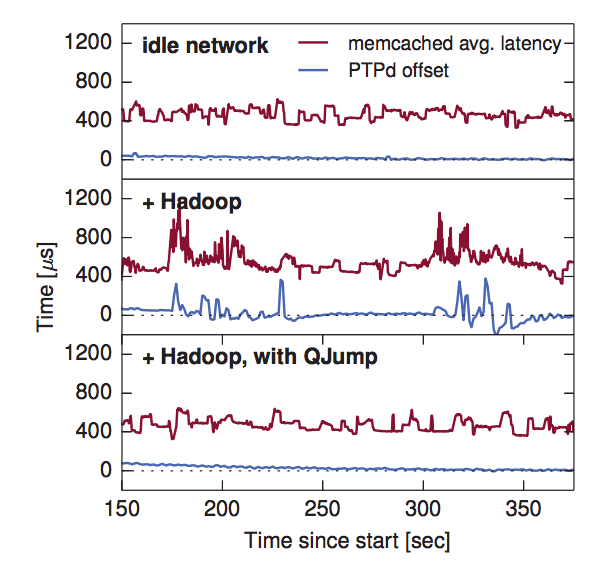
\includegraphics[width=200pt]{qjump.png} 
	
\section*{Current Progress}
	Thus far, we have created a mininet topology to mimic the original experimental topology and run some simple tests over it to gauge its viability in reproducing the experiment on shared hardware. For example, we have run PTPd between the virtual hosts and observed relatively small clock offsets. We have done extensive research on all of the underlying components of the experiment. We are also in correspondence with the author about replicating this experiment. The biggest design challenges of replicating this particular experiment on a virtual network involve scale and the use of shared hardware without a hardware abstraction. If applications like PTPd are particularly sensitive to jitter in the network, they will be heavily affected by virtualization overhead at both the hosts and the switches. Additionally, Hadoop suffers from a large ratio of baseline control traffic to generated high volume traffic as the scale of the cluster and the dataset being processed decreases. Hadoop will have to be configured to treat the single machine as if it were several instances of Hadoop running on different hosts by duplicating config files. This may be a very tricky problem.\\
	\\	
	 We have not yet attached the QJump kernel module to any of the mininet hosts because to do so we must first tackle several of the problems encountered by the team which replicated another experiment from this paper last year. The qjump-tc qdisc must be modified to support timing via the CPU clock rather than TSC and then subclassed to the existing mininet TC module.
	 
\subsection*{Plans}
	Without looking at any of their solution code, we have a pretty good idea of the work that needs to be done to get mininet nodes to support the use of QJump at all based on the challenges outlined in last year's result replication from the same paper. The kernel module must be modified and installed as a subclass, the Mininet hosts must be configured to use VLAN, the switches must be modified to use a fair scheduler if possible, and support must be added for multiple output queues. A possible alternative for multiqueue support would be to modify the qdisc to use a single queue at a given priority at each host if this is easier to implement. We will explore this possibility also. The first order of business is trying to get Hadoop to play nicely on a filesystem that it shares with itself. The biggest limitation here is that Hadoop uses configuration files to establish the directories used during operation and we need a way to alter the Hadoop configuration at each host to use different config files which point it to different tmpfs directories. Even if this can be accomplished we still have to figure out how to scale the Hadoop job down so that it generates enough cross-traffic but doesn't introduce too much background interference caused by control traffic. If using Hadoop over Mininet is intractable, we will try to find an alternative to generate unpredictable volumes of cross-traffic. Memcached should be relatively easy to scale down. We will reduce the number and size of requests generated by memaslap to some target latency and then scale up the request rate until it starts to affect latency.
		
\end{document}




